\documentclass{beamer}
\usepackage[utf8]{inputenc}
\usepackage[spanish]{babel}
\usepackage{natbib}
\usepackage{graphicx}
\usepackage{minted}
\usepackage{url}
\usepackage{caption}
\def\UrlBigBreaks{\do\/\do-\do:\do.}
\newcommand{\shellcmd}[1]{\\\indent\indent\texttt{\footnotesize\# #1}\\}
%Beamer theme
\usetheme{Madrid}

%Define minted environment for coding
\newminted{python}{fontsize=\scriptsize, 
                   linenos,
                   numbersep=5pt,
                   %gobble=4,
                   frame=lines,
                   framesep=2mm,
                   baselinestretch=1.1,
                   }
      
%Change frametitle color and add headline
\setbeamercolor{frametitle}{bg=gray!25}
\setbeamertemplate{headline}
{
   \leavevmode%
   \hbox{%
   \begin{beamercolorbox}[wd=.5\paperwidth,ht=2.25ex,dp=1ex,right]{section in head/foot}%
     \usebeamerfont{section in head/foot}\ \insertsectionhead\hspace*{2ex}
   \end{beamercolorbox}%
   \begin{beamercolorbox}[wd=.5\paperwidth,ht=2.25ex,dp=1ex,left]{subsection in head/foot}%
     \usebeamerfont{subsection in head/foot}\hspace*{2ex}\insertsubsectionhead
   \end{beamercolorbox}}%
   \vskip0pt%
}

%Title frame and footers
\title[Introducción a git]{\textbf{Introducción a git}}
\author[Nico Lois basado en apuntes de Risaro, D.]{Control de versiones con git \\ Repositorios remotos - gitHub}
\institute[]{}
\date{21/08/2020}

%-------------- BEGIN PRESENTATION ---------------%
\begin{document}
\maketitle

%%------------------------------------------------------------------------------%
\section{Sistemas de control de versiones (SCV)}
% FRAME
\begin{frame}{¿Qué es un CV?}

Llamamos \textbf{control de versiones} a una forma de gestionar los cambios que se realizan sobre documentos, programas o cualquier tipo de archivo. La idea de un \textbf{sistema de control de versiones} (SCV) es poder recuperar la versión  de cualquier archivo o documento en un estado anterior en el tiempo.\\

Algunos ejemplos de la vida real pueden ser:

\begin{itemize}
    \item Cuaderno de laboratorio 
    \item Revisiones de un artículo o tesis
    \item Desarrollo de un código (\textit{scripting})
\end{itemize}
\end{frame}

% FRAME
\begin{frame}{SCV}
\textbf{OK, y ¿para qué?}

\end{frame}

% FRAME
\begin{frame}{SCV}
\textbf{¿Para qué queremos realizar un CV?}
\begin{figure}
    \centering
    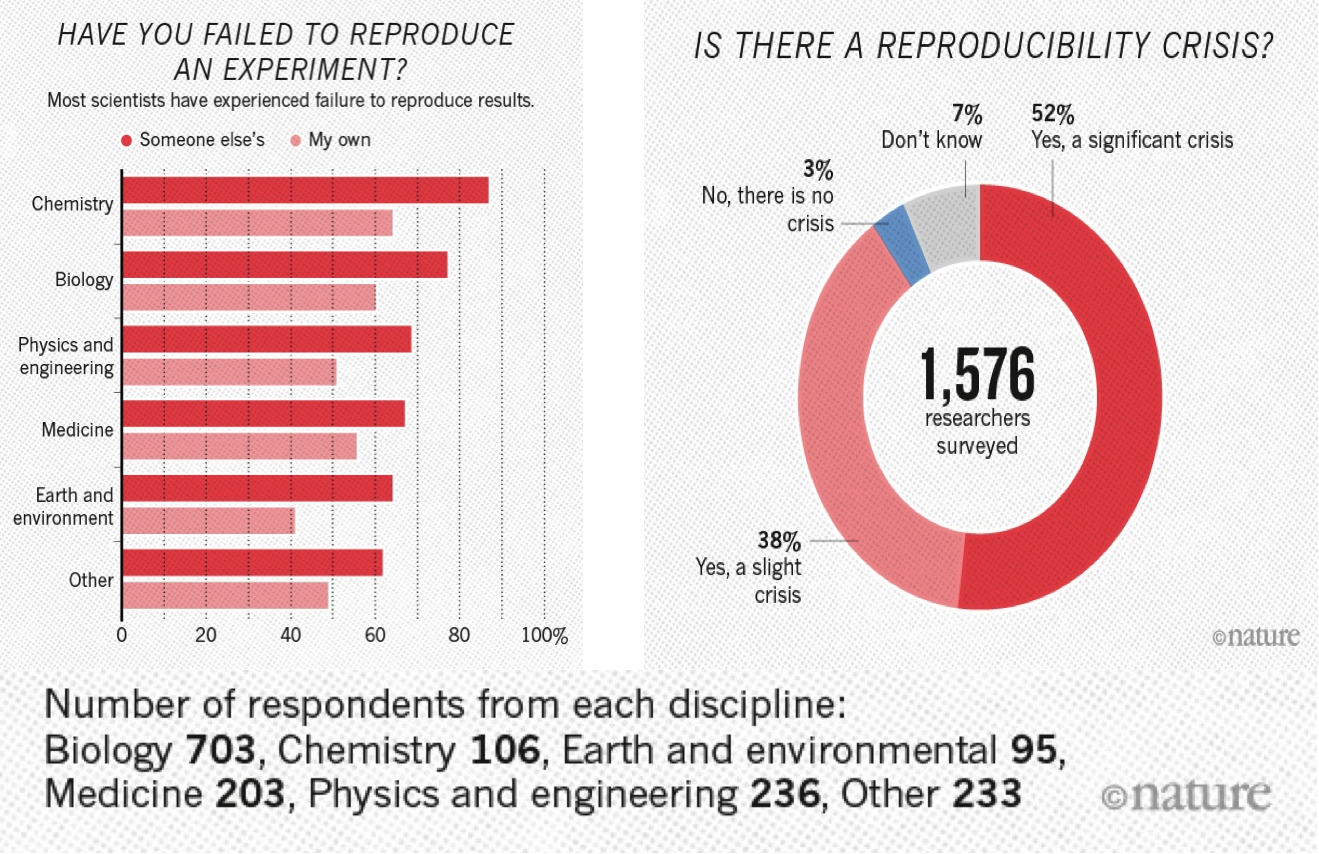
\includegraphics[scale=0.35]{reproducibility_nature.jpg}
\end{figure}
\end{frame}

% FRAME
\begin{frame}{SCV}
\textbf{¿Para qué queremos realizar un CV?}

\begin{figure}
    \centering
    
\includegraphics[scale=0.35]{SCV.png}
\end{figure}
\end{frame}

% FRAME
\begin{frame}{SCV}
\textbf{¿Para qué queremos realizar un CV?}
\begin{figure}
    \centering
    
\includegraphics[scale=0.35]{codigo.jpg}
\end{figure}
\end{frame}

% FRAME
\begin{frame}{SCV}
\textbf{¿Para qué queremos realizar un CV?}
\begin{figure}
    \centering
    
\includegraphics[scale=0.25]{reproducibility.png}
    
\includegraphics[scale=0.1]{reproducibilityESA.jpeg}
\end{figure}
\end{frame}


% FRAME
\begin{frame}{git}
¿Qué nos permite hacer \texttt{git}?
\begin{itemize}
    \item Tener backups en todos los estadíos de nuestro proyecto
    \item Documentar cambios
    \item Compartir cambios
    \item Distribuir el producto y el desarrollo a la vez a muchas personas
\end{itemize}
\end{frame}

% FRAME
\begin{frame}{git}
Algunos conceptos importantes

\begin{itemize}
    \item \textbf{Repositorios:} análogos a carpetas o conjunto de carpetas que conforman nuestro proyecto.
    \item  \textbf{Estados de un repositorio:} Conforma una imagen instantánea del proyecto. Cuando terminamos de trabajar en nuestro repositorio (carpeta), podemos consolidar los cambios realizados para no modificarlo más. Esto es como tomar un \textit{snapshot} del repo. El \textit{snapshot} actual se llama \texttt{HEAD}
    \item \textbf{Ciclo de vida de los archivos:} en un repo de \texttt{git} cada archivo puede tener uno de estos tres estados:
    \begin{itemize}
        \item no-modificado
        \item modificado
        \item actualizado
    \end{itemize}
\end{itemize}
\end{frame}

% FRAME
\begin{frame}{git}
\begin{figure}
    \centering
    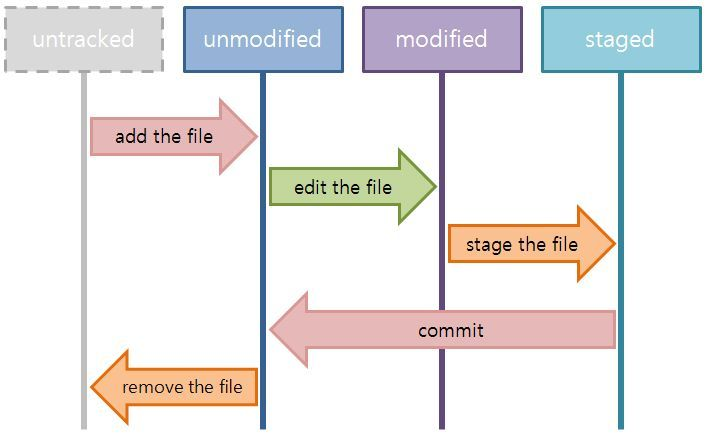
\includegraphics[scale=0.45]{file_lifecycle.jpg}
\end{figure}
\end{frame}


% FRAME
\begin{frame}{git}

\begin{itemize}
    \item Un archivo está en estado \textbf{no-modificado} cuando es igual al archivo guardado en el último \textit{snapshot}.
    \item Al modificar cualquier linea o caracter de un archivo, transforma al documento en un archivo \textbf{modificado}.
    \item El hecho de que un archivo esté modificado no implica que \texttt{git} haga un seguimiento automático del mismo. Hay que \textbf{actualizar} (en inglés, \textit{stage}) los archivos modificados para luego consolidar esos cambios, es decir, tomar un nuevo \textit{snapshot}.
    \item Al hacer esto, los archivos que estaban actualizados ahora forman parte del nuevo \textit{snapshot}, que pasa a ser el nuevo \texttt{HEAD} del repositorio. De esta manera, los archivos que se encontraban en el estado actualizado pasan al estado no-modificado.
    \item Finalmente, si creamos un archivo nuevo y le queremos dar seguimiento, tenemos que agregarlo al repositorio. De la misma forma, podemos remover un archivo del repo. 
\end{itemize}
\end{frame}


% FRAME
\begin{frame}{git (hands-on)}

  \noindent Primero, vamos a crear un directorio de trabajo:
  \shellcmd{mkdir ejercicio-git}
  
  \noindent Ahora sí, vamos al directorio de trabajo y creamos un repositorio:
  \shellcmd{cd ejercicio-git}
    \vspace{-.5cm}
  \shellcmd{git init}
  
  \noindent Esto genera una carpeta oculta dentro del directorio en el que estamos trabajando y lo podemos visualizar con los comandos:
  \shellcmd{ls -a}
  
  \noindent El estado del repositorio se consulta ejecutando:
  \shellcmd{git status}
  
\end{frame}

% FRAME
\begin{frame}{git (hands-on)}

  \noindent Dado que todavía no agregamos archivos para seguir en el repositorio, este comando nos dirá que el repositorio está vacío. \\ Ahora, creen/copien un archivo cualquiera en el directorio.
  \shellcmd{echo 'hola' > hola.txt}
  
  \noindent ¿Cómo iniciamos el seguimiento de archivos?
  \shellcmd{git add .}

  \noindent Una vez que empezamos a seguir todos los archivos en la carpeta debemos \textit{consolidar} los cambios:
  \shellcmd{git commit -m  $"$Agrego un archivo al repositorio$"$}
  
  \noindent Cada \textit{commit} tiene un \textit{hash}, que es un número hexadecimal con el que se reconoce unívocamente el \textit{snapshot} que estamos tomando. En mi caso:
  \shellcmd{0ae96ca09bb0293af61e3e8a6de1a198a8c6459f}
\end{frame}

% FRAME
\begin{frame}{git (hands-on)}
  \noindent Si ahora consultamos el estado del repositorio:
  \shellcmd{git status}

  \shellcmd{nothing to commit, working tree clean}

El mensaje nos dice que no hay archivos en estado
modificado, ya que el archivo que agregamos antes (y que no volvimos a modificar) es
igual al que está guardado en HEAD.
\end{frame}

% FRAME
\begin{frame}{git (hands-on)}
Ahora, la tarea para generar un \textit{snapshot} es siempre la misma:
\begin{itemize}
    \item Modificamos/creamos uno o varios archivos.
    \item Los agregamos al staging area con \texttt{git add . }
    \item Los consolidamos en un snapshot con \texttt{git commit -m $"$mensaje$"$}
\end{itemize}
\vspace{1cm}
\textcolor{orange}{Entonces ahora agreguen/creen un par de archivos más y hagan otro  \texttt{commit} }


\end{frame}

\begin{frame}{git (hands-on)}
\noindent Podemos a todo momento consultar el historial de \textit{commits} realizados en el repositorio:
\shellcmd{git log}
\shellcmd{commit 0ae96ca09bb0293af61e3e8a6de1a198a8c6459f (HEAD -> master, origin/master)}
  \vspace{-.5cm}
\shellcmd{Author: Nico Lois <nico.harry.lois@gmail.com>}
  \vspace{-.5cm}
\shellcmd{Date:   Tue Jul 28 16:59:12 2020 -0300}
  \vspace{-.5cm}
\shellcmd{agrego archivo}

Cada commit tendrá un código con el cual uno puede ir a \textit{snapshots} viejos:

\shellcmd{git checkout <commit hash>}

En mi caso:
\shellcmd{git checkout 9f8b}
\end{frame}


\begin{frame}{git: Ramas (Branches)}
Hasta ahora, nuestro trabajo puede resumirse en una línea de tiempo de este estilo:
\begin{figure}
    \centering
    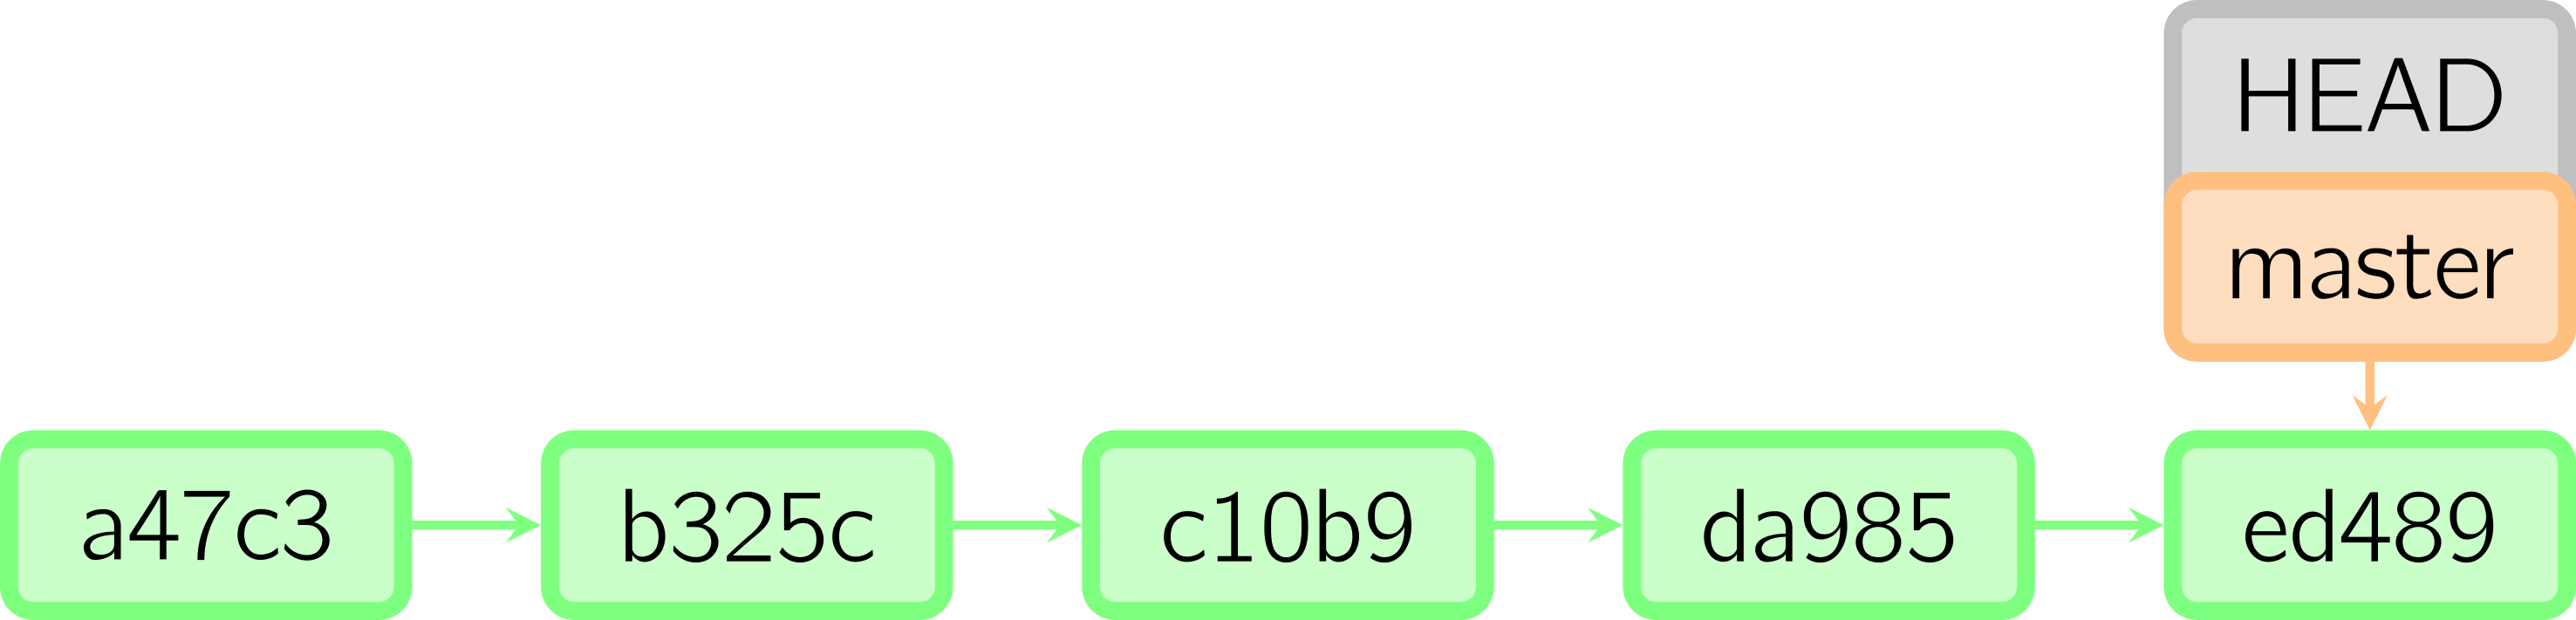
\includegraphics[scale=0.65]{master.png}
\end{figure}

El trabajo se realizó siempre en la rama \textit{master}
\end{frame}


\begin{frame}{git: Ramas (Branches)}
Ahora veamos cómo implementar cambios grandes que pueden comprometer la funcionalidad general de todo el repositorio. Por ejemplo, agregar una nueva funcionalidad
\begin{itemize}
    \item graficar una serie de variables
    \item agregar un paquete de análisis nuevo.
\end{itemize}

\begin{figure}
    \centering
    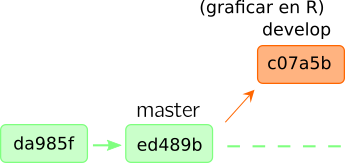
\includegraphics[scale=0.65]{branch.png}
\end{figure}

\end{frame}

\begin{frame}{git: Ramas (Branches)}
\noindent Con \texttt{git} podemos dar siguimiento a una nueva rama de la siguiente manera: 
generamos una rama llamada \textbf{develop} y nos posicionamos en esa rama

\shellcmd{git branch develop}
  \vspace{-.5cm}
\shellcmd{git checkout develop}
Luego, seguimos trabajando de la misma manera que vimos anteriormente, y los \textit{commits}, se realizarán sobre la rama \textbf{develop} y la rama \textbf{master} no tendrá \textit{commits}.
\begin{figure}
    \centering
    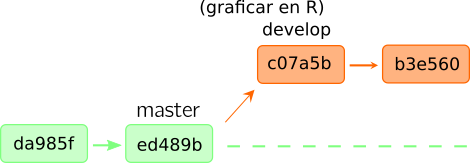
\includegraphics[scale=0.5]{branch_develop.png}
\end{figure}
\end{frame}

% \begin{frame}{git: ramas}
% \noindent Realizamos esto con \texttt{git} de la siguiente manera: 
% generamos una rama llamada \textbf{grafico} y nos posicionamos en esa rama

% \shellcmd{git branch grafico}
%   \vspace{-.5cm}
% \shellcmd{git checkout grafico}
% Luego, seguimos trabajando de la misma manera que vimos anteriormente, y los \textit{commits}, se realizarán sobre la rama \textbf{grafico} y la rama \textit{master} no tendrá \textit{commits}.
% \begin{figure}
%     \centering
%     \includegraphics[scale=0.5]{branch_2.png}
% \end{figure}
% \end{frame}


\begin{frame}{git: Ramas (Branches)}
\noindent El siguiente paso será juntar estar dos implementaciones (al fin y al cabo,
es lo que queremos). Para eso, debemos unir las dos ramas.

\shellcmd{git merge master develop}
\begin{figure}
    \centering
    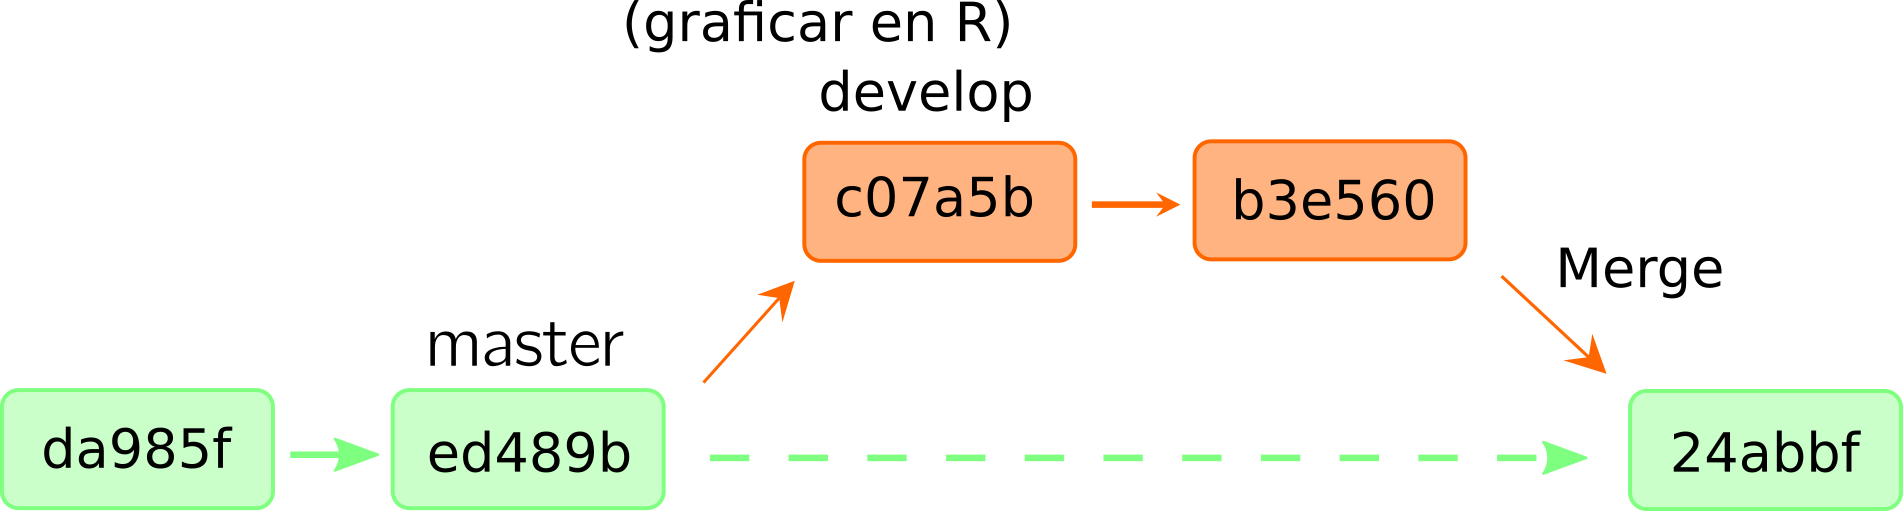
\includegraphics[scale=0.5]{branches.png}
\end{figure}
\end{frame}

\begin{frame}{git: repositorios remotos}
El último paso es poder comunicarnos con un repositorio remoto

\begin{itemize}
    \item Crear un usuario en \texttt{github.com}
    \item Crear un repositorio en github, que llamaremos \texttt{ejercicio-git}, la dirección del repo será: \texttt{https://github.com/<USUARIO>/ejercicio-git.git}
    \item Nos comunicamos con el repositorio remoto: \texttt{git remote add origin https://github.com/dbrisaro/ejercicio-git.git}
    \item \textit{Pusheamos} los cambios del local al remoto \texttt{git push -u origin master}
    \item Si estamos colaborando, puede el repositorio remoto tener cambios que no están en el local, para eso realizamos \texttt{git pull origin master}
    
\end{itemize}
\end{frame}

\begin{frame}{git: repositorios remotos}
Algo que solemos hacer es querer utilizar repositorios remotos públicos. Hay varias formas para obtener los repositorios:

\begin{figure}
    \centering
    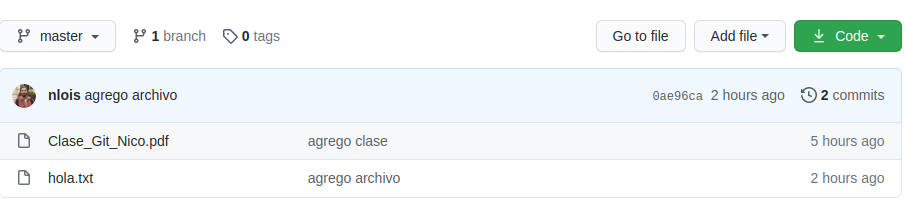
\includegraphics[scale=0.3]{github_download.png}
\end{figure}

\begin{itemize}
    \item Abrir el archivo en el repositorio remoto y copiarlo.
    \item Descargar el repositorio desde el botón verde \textbf{Code}
    \item Utilizar una línea de comando
\end{itemize}
\shellcmd{git clone https://github.com/nlois/ejercicio-git.git}

\end{frame}
\end{document}